% example.tex
\documentclass[dvisvgm]{standalone}
\usepackage{pgfplots}
\pgfplotsset{
    width=5cm, 
    legend style={
        font=\footnotesize,
        %rounded corners=2pt
    },
    compat=newest
}
\usepgfplotslibrary{groupplots,dateplot}
\usetikzlibrary{patterns,shapes.arrows}
\usetikzlibrary{decorations.pathreplacing,calligraphy}
\begin{document}
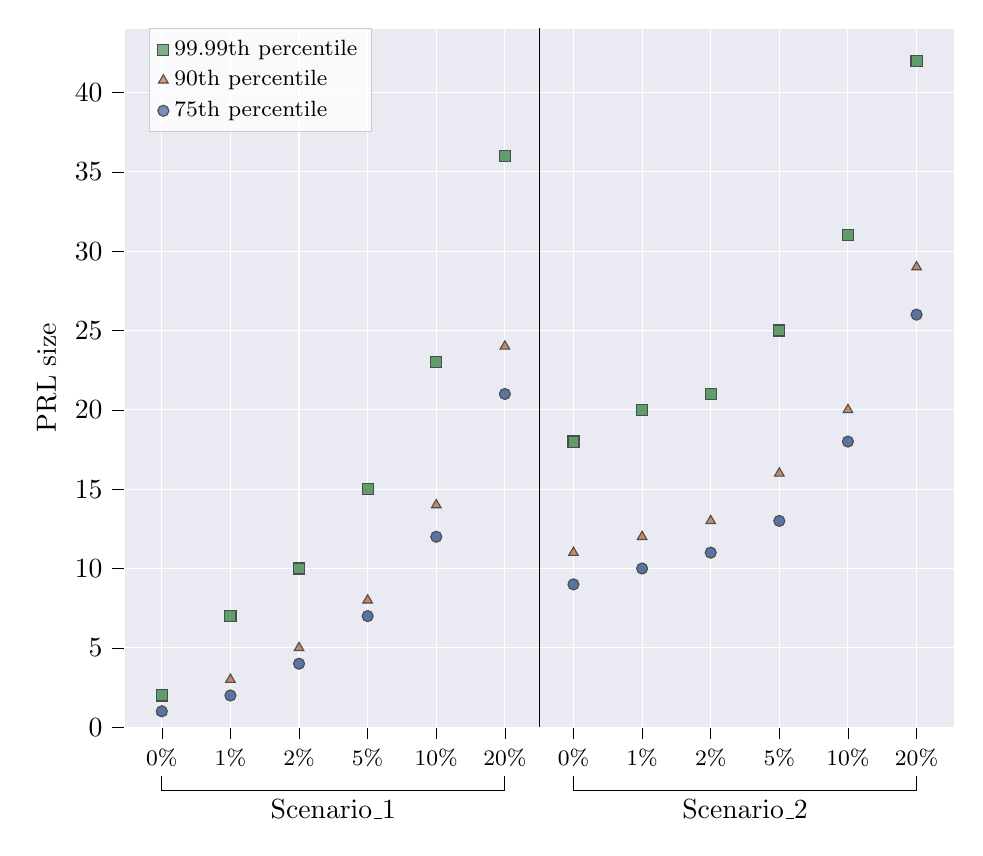
\begin{tikzpicture}

    \definecolor{lightgray204}{RGB}{204,204,204}
    \definecolor{darkslategray38}{RGB}{38,38,38}
    \definecolor{darkslategray76}{RGB}{76,76,76}
    \definecolor{indianred1819295}{RGB}{181,92,95}
    \definecolor{lavender234234242}{RGB}{234,234,242}
    \definecolor{lightslategray133122170}{RGB}{133,122,170}
    \definecolor{mediumseagreen95157109}{RGB}{95,157,109}
    \definecolor{peru20313699}{RGB}{203,136,99}
    \definecolor{steelblue76114176}{RGB}{76,114,176}
    \definecolor{steelblue88116163}{RGB}{88,116,163}
    
    \begin{axis}[
      width=\columnwidth,
      ylabel= PRL size,
      xmajorgrids,
      xmajorticks=true,
      ymajorgrids,
      ymajorticks=true,
      axis background/.style={fill=lavender234234242},
      axis line style={white},
      x grid style={white},
      y grid style={white},
    legend cell align={left},
    legend style={
      fill opacity=0.8,
      draw opacity=1,
      text opacity=1,
      at={(0.03,1.0)},
      anchor=north west,
      draw=lightgray204
    },
    tick align=outside,
    tick pos=left,
    % x grid style={darkgray176},
    xmin=-0.55, xmax=11.55,
    xtick style={color=black},
    xtick={0,1,2,3,4,5,6,7,8,9,10,11},
    xticklabel style={name=tick no \ticknum, font=\footnotesize},
    xticklabels={
      $0\%$,
      $1\%$,
      $2\%$,
      $5\%$,
      $10\%$,
      $20\%$,
      $0\%$,
      $1\%$,
      $2\%$,
      $5\%$,
      $10\%$,
      $20\%$
    },
    % y grid style={darkgray176},
    ymin=0.0, ymax=44.05,
    ytick style={color=black}
    ]
    \addplot [draw=darkslategray76, fill=mediumseagreen95157109, mark=square*, only marks]
    table{%
  x  y
  0 2
  1 7
  2 10
  3 15
  4 23
  5 36
  6 18
  7 20
  8 21
  9 25
  10 31
  11 42
  };
  \addlegendentry{99.99th percentile}
  \addplot [draw=darkslategray76, fill=peru20313699, mark=triangle*, only marks]
  table{%
  x  y
  0 1
  1 3
  2 5
  3 8
  4 14
  5 24
  6 11
  7 12
  8 13
  9 16
  10 20
  11 29
  };
  \addlegendentry{90th percentile}
  \addplot [draw=darkslategray76, fill=steelblue88116163, mark=*, only marks]
  table{%
  x  y
  0 1
  1 2
  2 4
  3 7
  4 12
  5 21
  6 9
  7 10
  8 11
  9 13
  10 18
  11 26
  };
  \addlegendentry{75th percentile}
  
  \draw (axis cs:5.5,0) -- (axis cs:5.5,45);
  
  % \draw (axis cs:0.0, -2) -- (axis cs:0.0, -4) -- (axis cs:5.0, -4) -- (axis cs:5.0, -2);
  
  
  \end{axis}
  \draw  (tick no 0.south) -- +(0,-.5em) -- ([yshift=-.5em] tick no 5.south)  node [midway, below] {Scenario\_1}  -- +(0,.5em);
  \draw  (tick no 6.south) -- +(0,-.5em) -- ([yshift=-.5em] tick no 11.south) node [midway, below] {Scenario\_2} -- +(0,.5em);
    
    \end{tikzpicture}
\end{document}